\documentclass{article}




\usepackage[english]{babel}
\usepackage{float}
\usepackage{tabularx}
\usepackage{parskip} 
\usepackage{mathtools}
% Set page size and margins
% Replace `letterpaper' with`a4paper' for UK/EU standard size
\usepackage[letterpaper,top=2cm,bottom=2cm,left=3cm,right=3cm,marginparwidth=1.75cm]{geometry}

% Useful packages
\usepackage{amsmath}
\usepackage{graphicx}
\usepackage[colorlinks=true, allcolors=blue]{hyperref}

%\title{DevOps, Software Evolution and Software Maintenance}
\begin{document}
\title{%
  DevOps, Software Evolution and Software Maintenance (BSDSEMSM1KU) \\
  \large Group H - Neutrals}

\author{Alekxander Baxwill (abax@itu.dk)\\ \\ Jacob Sjöblom (jsjo@itu.dk) \\ \\ Frederik Peter Volkers (frvo@itu.dk) \\ \\ Albert Bethlowsky Rovsing (arov@itu.dk) \\ \\ Rasmus Andreas de Neergaard (rade@itu.dk) \\ \\ Repository: \url{https://github.com/albertbethlowsky/DevOpsGroupH}} 



\maketitle


%Title:
%\maketitle
\begin{figure}[H]
\centering
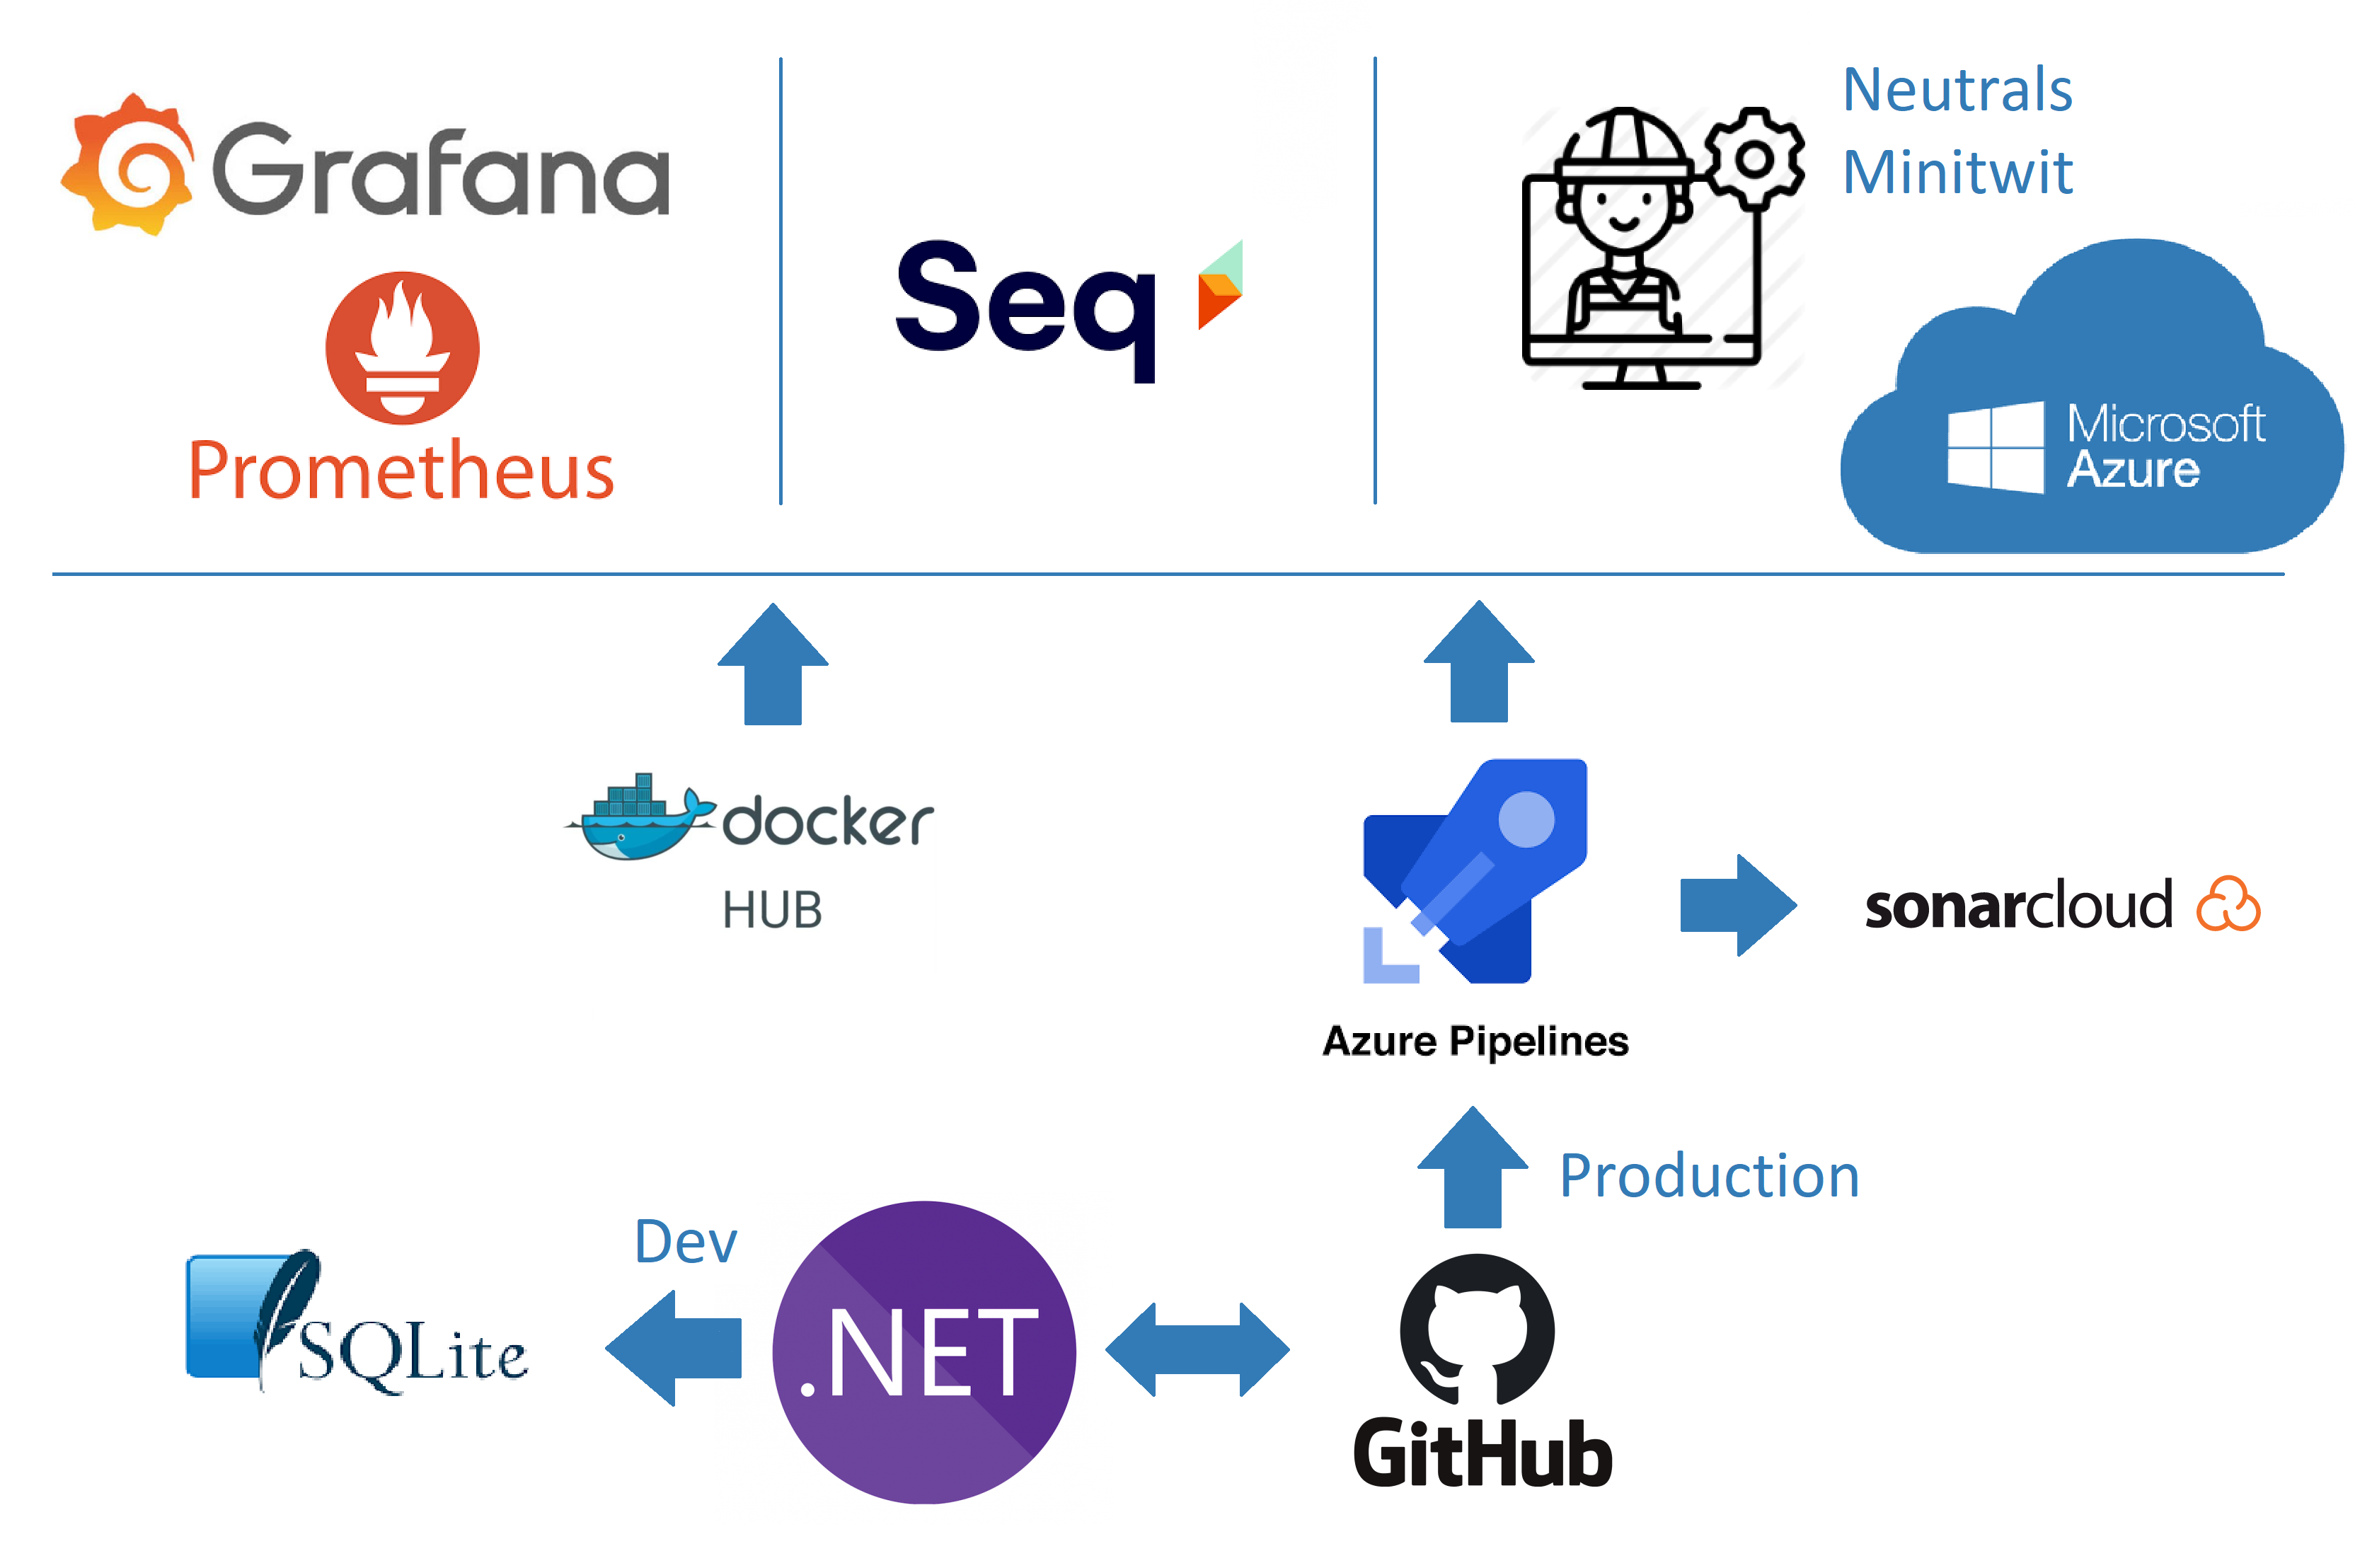
\includegraphics[width=1\textwidth]{images/SystemDesign.png}
\end{figure}
\newpage

%Table of contents:
\tableofcontents
\newpage

%Checklist/skeleton: https://github.com/itu-devops/lecture_notes/blob/master/REPORT.md
% revised idea for skeleton:
\newpage
\section{System's Perspective}
% skriv hvorfor vi vælgeer c# azure og asp.net
\subsection{Design and Architecture of the system}
In the beginning we decided on rebuilding the solution with the language C\#. As an alternative Java was also discussed, since everyone in the group have previous experience with it. We decided on C\# over Java to give ourselves an opportunity to explore a new language, while still having some experience to fall back on due to the similarities between the two. In addition C\# is widely used in the industry, and gaining experience with .NET could be a good addition to our future job aspects.

For the cloud provider, Digital Ocean was initially considered but we decided on Microsoft Azure, due to the synergy between Azure and other Microsoft Services (Azure DevOps, Azure SQL, Monitoring etc.), in addition, some team members have prior experience with Azure. Azure also provides students with free credits.

For the backend we decided on ASP.NET Core MVC which uses the Model-View-Controller architectural pattern. For the object relational mapper (ORM), Microsoft’s Entity Framework Core (EF Core) was used. Other common options are NHibernate or Linq2Db. EF Core has great documentation, was simple to integrate and is popular with .NET web applications. In relation to choosing the DBMS, MySQL was considered due to it being open source and popular in general. We however opted for Azure SQL Server (db as a service) because it's easy to scale, setup and comes with neat features such as AI optimised queries etc.

For an overview of the architecture and design of the MiniTwit application, the 3+1 approach is used. 

\subsubsection*{Module View}
\begin{figure}[H]
\centering
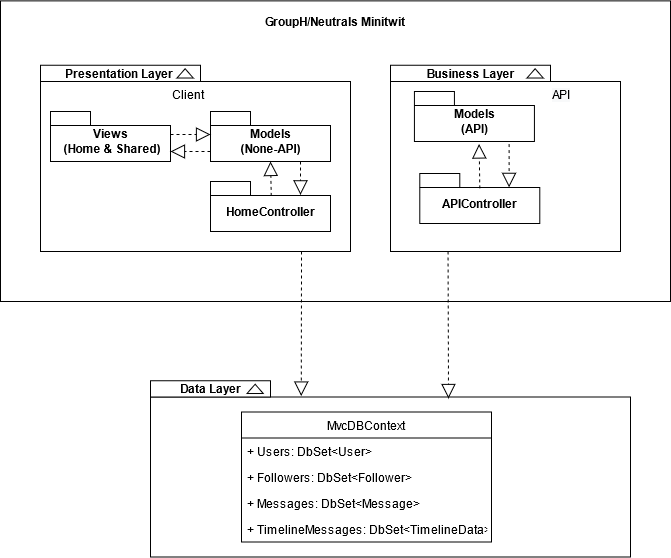
\includegraphics[width=0.7\textwidth]{images/Module View (3+1).png}
\caption{\label{fig:modview} Module View}
\end{figure}

Fig. \ref{fig:modview} illustrates the relations between the packages at design time.
Presentation Layer highlights the flow of information via the MVC model based on user interaction. User input in any view is translated into a model object, fed into the HomeController. The targeted action is processed by the controller and output is distributed back to the view via a model object, providing a dynamic user interface, which is not included in the Module view.
The Business layer is built on the same principle, but does not include a view. %In addition to returning data to the view, the Models also communicate attributes needed to be retained in the Data Layer for specific actions, which 
For data retention, model objects are translated to SQL and executed by EF Core on the db. 

\subsubsection*{Component \& Connector View}
\begin{figure}[H]
\centering
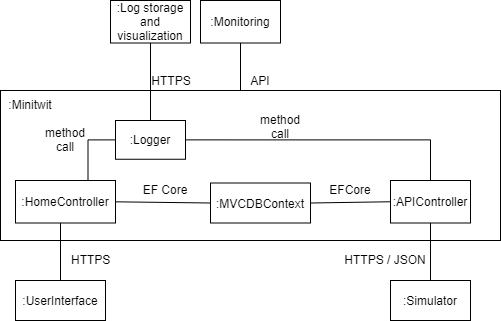
\includegraphics[width=0.9\textwidth]{images/ccview.png}
\caption{\label{fig:ccview}Connector and Component View}
\end{figure}
Fig. \ref{fig:ccview} illustrates how the system interacts between its components at runtime. It is worth mentioning that Logger is a default extension of the framework where Serilog is injected on top at startup.

\subsubsection*{Deployment View}
\begin{figure}[H]
\centering
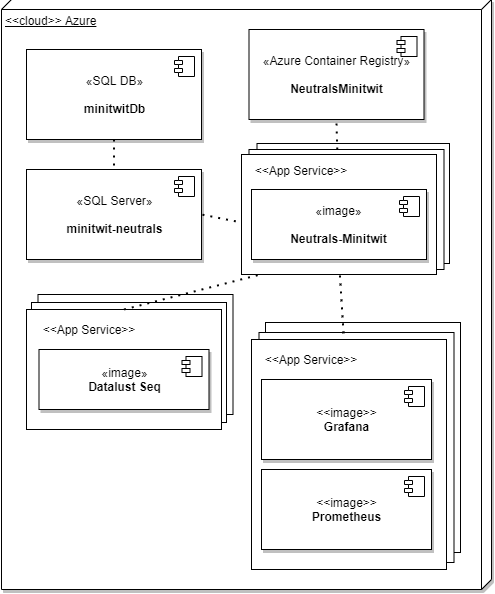
\includegraphics[width=0.6\textwidth]{images/Deployment View Point.png}
\caption{\label{fig:dview}Deployment View}
\end{figure}

Fig. \ref{fig:dview} illustrates the system at it's deployed state. 
\begin{itemize}
    \item $\ll$cloud$\gg$: Refers to the hosting of our services through Azure.
    \item $\ll$App Service$\gg$: Service hosting the images
    \item $\ll$Azure Container Registry$\gg$: Repository for the NeutralsMiniTwit images
    \item Neutrals-Minitwit image: The front- and back-end (API and server) of MiniTwit.
    \item Grafana image: Collects PromQL data from Prometheus, enabling visualization of metrics data.
    \item Prometheus image: Collects the exposed metrics of MiniTwit, and translates it into PromQL readable by Grafana.
    \item DataLust Seq image: Aggregates and stores logs sent from MiniTwit hosted in an App Service.
    \item $\ll$SQL Server$\gg$ and $\ll$SQL DB$\gg$: Azure hosted SQL Server with underlying database, used for persisting data used by the system.
\end{itemize}
NB: Worth noting, the App Services Neutrals-MiniTwit, Datalust Seq and (Grafana and Prometheus) are part of two separate service plans which are balanced between 3 VM's each. 

\newpage
\subsection{Dependencies}
\subsubsection{Software dependencies}
The dependencies of the system are derived via GitHub from the \texttt{mvc-minitwit.csproj} and \texttt{HomeControllerTests.csproj} project files, as seen in fig. \ref{fig:gitd}. These correspond to the MiniTwit and testing project respectively \cite{GitDepend}. 

\begin{figure}[H]
\centering
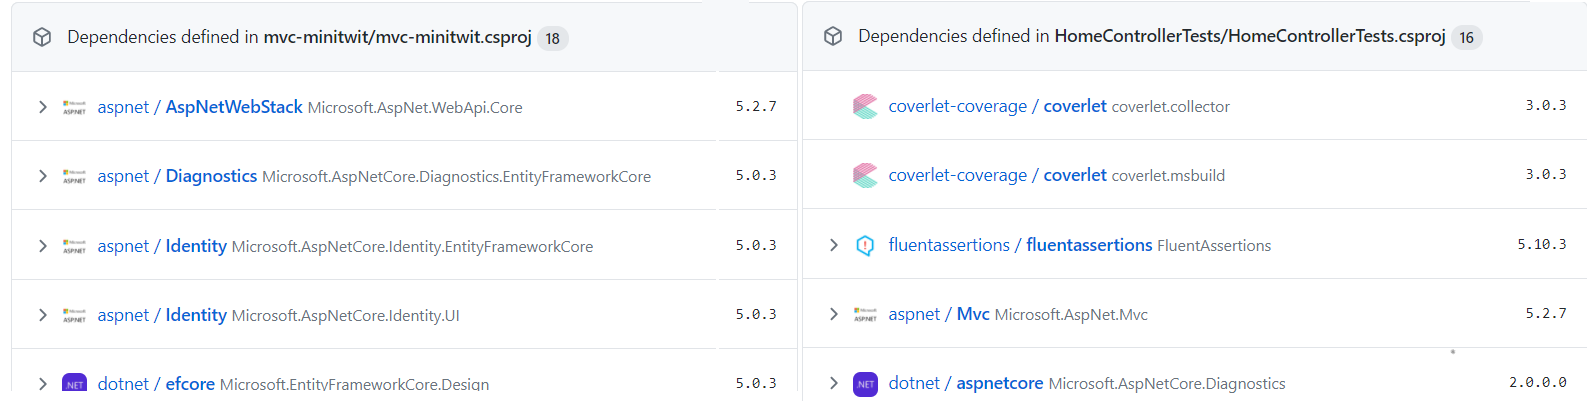
\includegraphics[width=1.1\textwidth]{images/dependencies-snip.png}
\caption{Snippet of GitHub dependency graph}
\label{fig:gitd}
\end{figure}

Additionally, using NDepend, we can provide a more detailed visualization of the dependencies. It is a static analysis tool which generates a dependency matrix for the backend dependencies. From the snippet of the matrix \ref{fig:matrix}, we can observe that the \emph{'mvc-minitwit'} package (row) is used by 20 code elements (blue) in \emph{'mvc-minitwit.Views'} (column) and \emph{'mvc-minitwit'} (column) is using 5 code elements (green) from \emph{'mvc-minitwit.Views'} (row) \cite{Ndepend}. This matrix does not include test dependencies. See GitHub repos for full image. 
\begin{figure}[H]
\centering
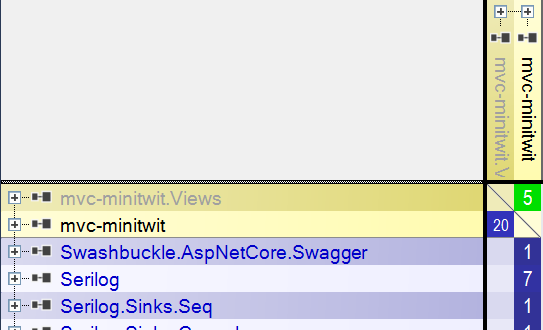
\includegraphics[width=0.7\textwidth]{images/ndepenmatrix.png}
\caption{\label{fig:matrix} Snippet of Ndepend - Dependency Matrix}
\end{figure}

\subsubsection{Cloud dependencies}
These non-repository dependencies are related to the services hosted on cloud-based domains.

\begin{table}[H]
\begin{tabularx}{\textwidth}{|l|l|l|X|}
\hline
    \textbf{Name} & \textbf{Service} & \textbf{Provider} & \textbf{Description} \\ \hline
    neutrals-minitwit & App Service & Microsoft Azure & development, rollout and scaling of web apps (.NET application) \\ \hline
    minitwit-neutrals & App Service & Microsoft Azure &development, rollout and scaling of web apps (prometheus, grafana) \\ \hline
    neutralsseq & App Service & Microsoft Azure & development, rollout and scaling of web apps (Datalust - Seq) \\ \hline
    minitwit-neutrals & SQL Server & Microsoft Azure & Hosting of SQL database \\ \hline
    minitwitDb & SQL database & Microsoft Azure & SQL database \\ \hline
    ASP-NeutralsRG & App Service Plan & Microsoft Azure & Hosting of Web Services (.NET application and Datalust - Seq) \\ \hline
    ASP-mvcminitwit & App Service Plan & Microsoft Azure & Hosting of Web Services (Grafana and Prometheus) \\ \hline
\end{tabularx}
\end{table}

%how does components talk together.. e.g. Sequence diagrams
\subsection{Current state of the system} 
With the help of different static analysis tools, it's possible to get a sense of the state of the system, including an estimation of the technical debt. Their respective results are briefly stated in following sections.

\subsubsection*{SonarCloud}
As observed from Fig. \ref{fig:sonar}, SonarCloud seems to be in a satisfactory state, however, there are a few caveats to point out. The auto-generated contents of \texttt{Migrations/}, and the \texttt{wwwroot/lib} folder has been excluded from all analysis since the latter contains deprecated jQuery libraries. These were given from the beginning, and were thus deemed out of scope to fix with time available. 

\begin{figure}[H]
\centering
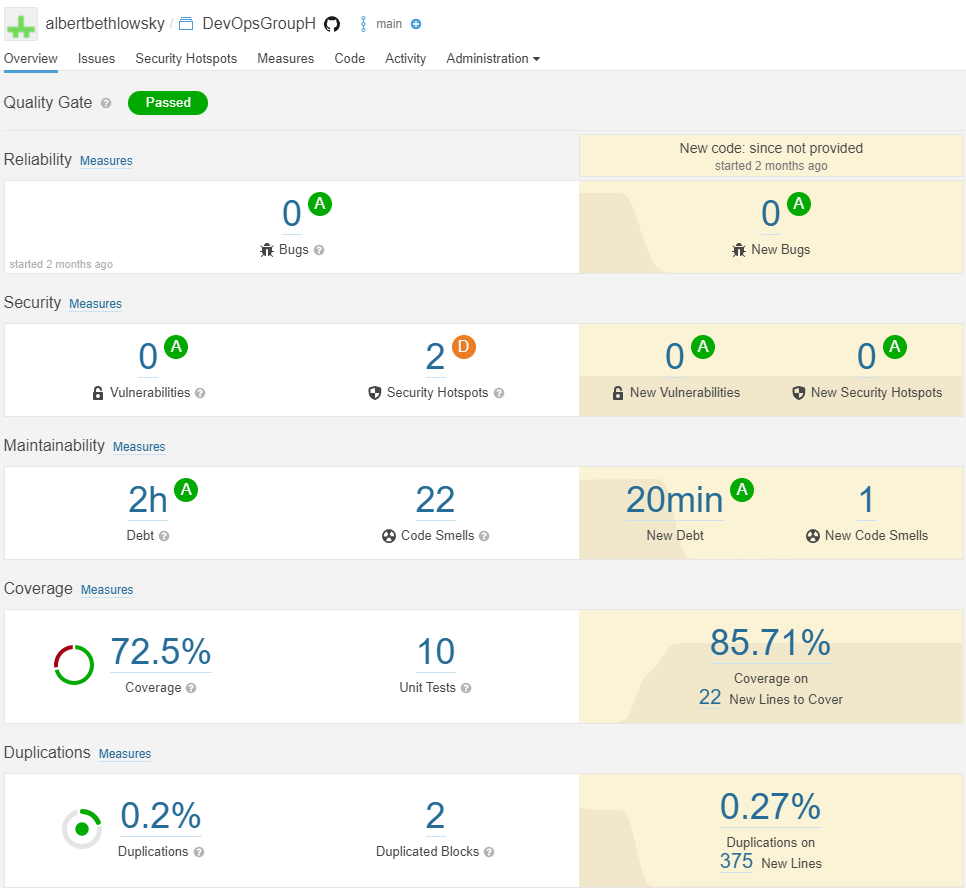
\includegraphics[width=0.7\textwidth]{images/sonarcloud.png}
\caption{\label{fig:sonar} Results from SonarCloud}
\end{figure}

The boiler plate, initialization files \texttt{Program.cs}, \texttt{Startup.cs} are excluded from test coverage analysis. \texttt{HomeController.cs} is also excluded from test coverage due to project scope and challenges with mocking cookies.
% her antages at læser ved hvad HomeController.cs er
From the maintainability category, there's "2 hours" of debt, but it's worth mentioning that it's a relative estimate based on "Code smells", uncovered and duplicated lines. This estimate should be compared with estimates from the other tools.   
\subsubsection*{Code Climate}
The repository has a maintainability grade of "B" as seen in Fig. \ref{fig:clim}, which with their estimates would be about 2 days of technical debt. There are 19 issues in total, split into 8 of duplication and 11 code smells. The file with the lowest maintainability score is \texttt{HomeController.cs} and has a "C", which would be the file to prioritize first for refactoring. The same files and folders have been excluded as with SonarCloud. %check this

As a side note a big source of the issues in both \texttt{HomeController.cs} and \texttt{APIController.cs} comes in the shape of \textit{"Avoid too many return statements"}. Arguably, this could be related to the debate of "clean OOP" approach, which is harder to implement in a server/API application. %let me know if u agree/disagree here  


\begin{figure}[H]
\centering
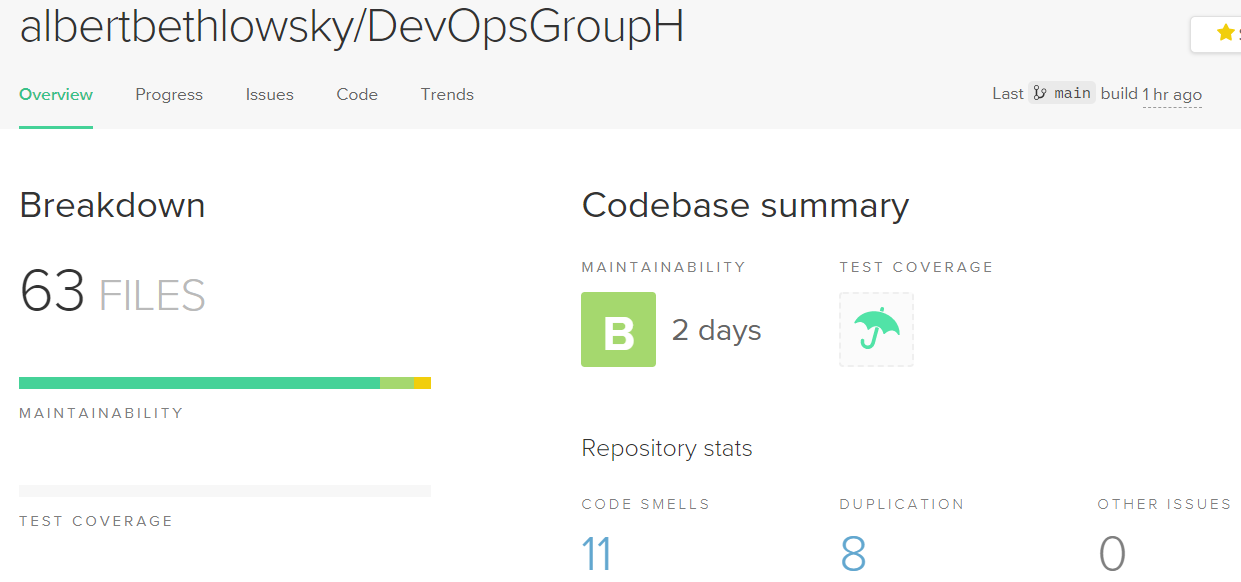
\includegraphics[width=0.7\textwidth]{images/codeclimate.png}
\caption{\label{fig:clim} Code Climate summary and overview}
\end{figure}

\subsubsection*{Better Code Hub}
We can observe from Fig. \ref{fig:code}, that our compliance is 7/10 and the code smells are similar to previous. We acknowledge that our lack of experience with C\# has some effects on our coding style. 

\begin{figure}[H]
\centering
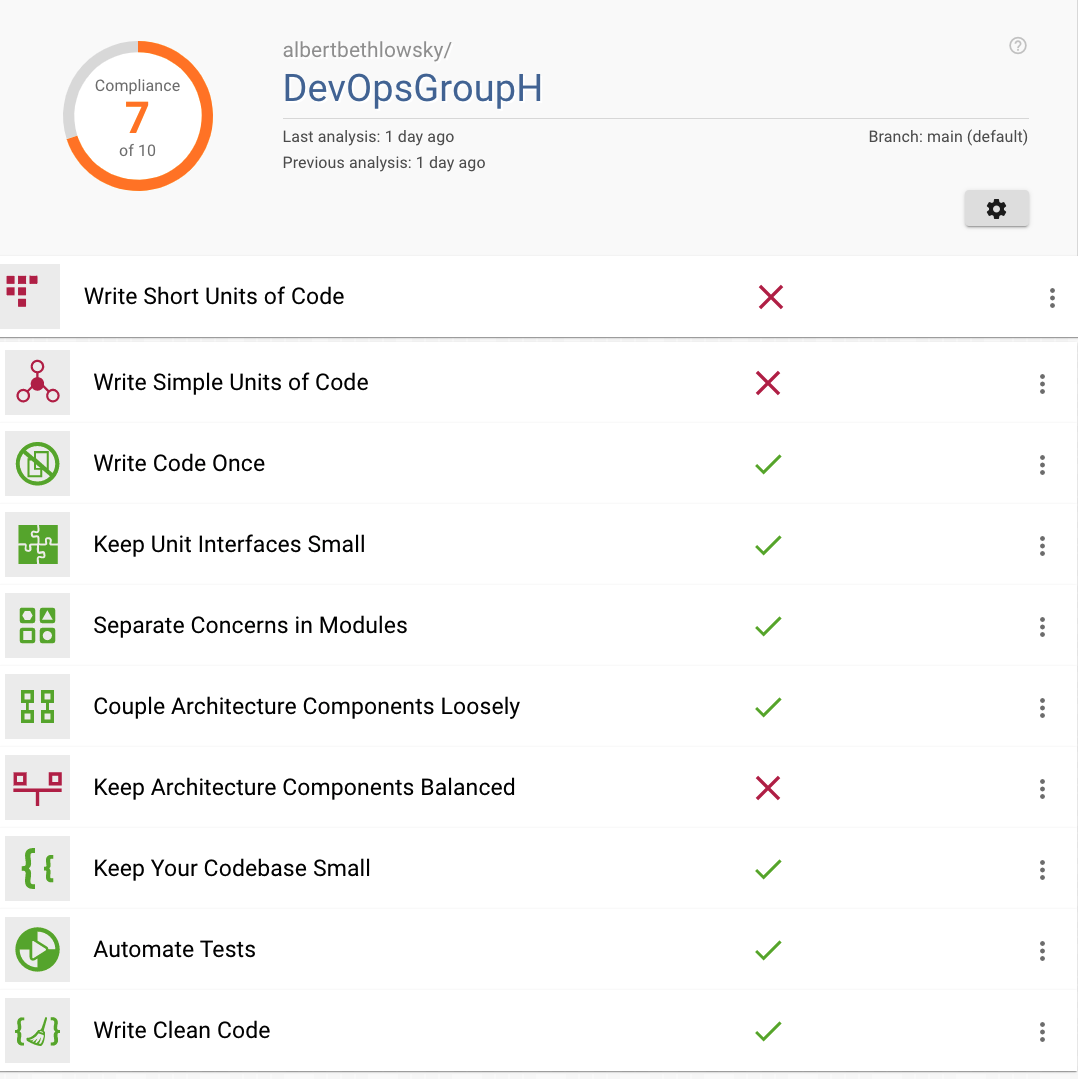
\includegraphics[width=0.7\textwidth]{images/bch.png}
\caption{\label{fig:code} Better Code Hub results}
\end{figure}

It's worth noting that technical debt is a relative term, and as seen between the tools, can vary quite a lot (e.g. 2 days to 2 hours).

\subsection{Licenses and compatibility}
The dependencies in our project are licensed under three licenses. The Apache 2.0 license \cite{apache}, the MIT license \cite{MIT} and the BSD-3 clause  \cite{BSD}. All of these licenses fall within the category of permissive licenses. 
The following table \ref{table:lic} shows how the dependencies are distributed on these different licenses. 
\begin{table}[H]
    \small
    \begin{tabular}{|l|l|l|l|}
        \hline
        Apache 2 License                            & MIT License                 & BSD 3      \\ \hline
       Aspnet/AspNetWebStack                  & Coverlet-coverage/coverlet    & Moq4/moq4      \\
       Aspnet/Diagnostics                     & Microsoft/vstest              &                \\
       Aspnet/hosting                         & Newtonsoft.Json               &                \\
       Aspnet/Identity                        & prometheus-net/prometheus-net &                \\
       Aspnet/Logging                         & Swashbuckle.AspNetCore        &                \\
       Aspnet/Mvc                             & Swashbuckle.AspNetCore        &                \\
       Dotnet/efcore                          &                               &                \\
       Donet/scaffolding                      &                               &                \\
       Serilog/serilog-aspnetcorer            &                               &                \\
       Serilog/serilog-filters-expressions    &                               &                \\
       Serilog/serilog-settings-configuration &                               &                \\
       Serilog/serilog-sinks-file             &                               &                \\
       Serilog/serilog-sinks-seq              &                               &                \\
       Fluentassertions/fluentassertions      &                               &                \\
       Xunit/xunit                            &                               &                \\
       Xunit/visualstudio.xunit               &                               &                \\
                                                                                                \hline
    \end{tabular}
    \label{table:lic}
\end{table}

All licenses impose no restrictions for us as we do not modify the source code of the dependencies. We have chosen Apache 2.0 as our license, since all licenses fall into the same category, and Apache 2.0 being most used. 

\section{Process perspective}
\subsection{Interactions between developers and organization}
As everyone in the team have different schedules it was difficult to find time to always meet fully. We strove towards having two weekly meetings on Mondays and Wednesdays. The communication and meetings were held online exclusive on Teams, and in each meeting we planned and presented progress. We assigned ourselves to tasks using GitHub Project Management. Often times team members would collaborate and do pair/group programming via VSCode Live Share.

\subsection{Description of CI/CD pipelines, stages and tools}
Azure DevOps is used to manage the CI/CD pipelines for the project. Azure DevOps was picked since it was easy to use and integrated well with hosting on Azure. As an example, certain services (Azure Kubernetes Services, Azure App Service for deployment, etc.) allowed for direct yaml-template injection via the marketplace on Azure DevOps.

There are two pipelines; the CI pipeline used for testing, code analysis, and building as seen in Fig \ref{fig:res}. And the CD pipeline for deploying as seen in Fig. \ref{fig:release}. 

\subsubsection*{Continuous Integration}
\begin{figure}[H]
\centering
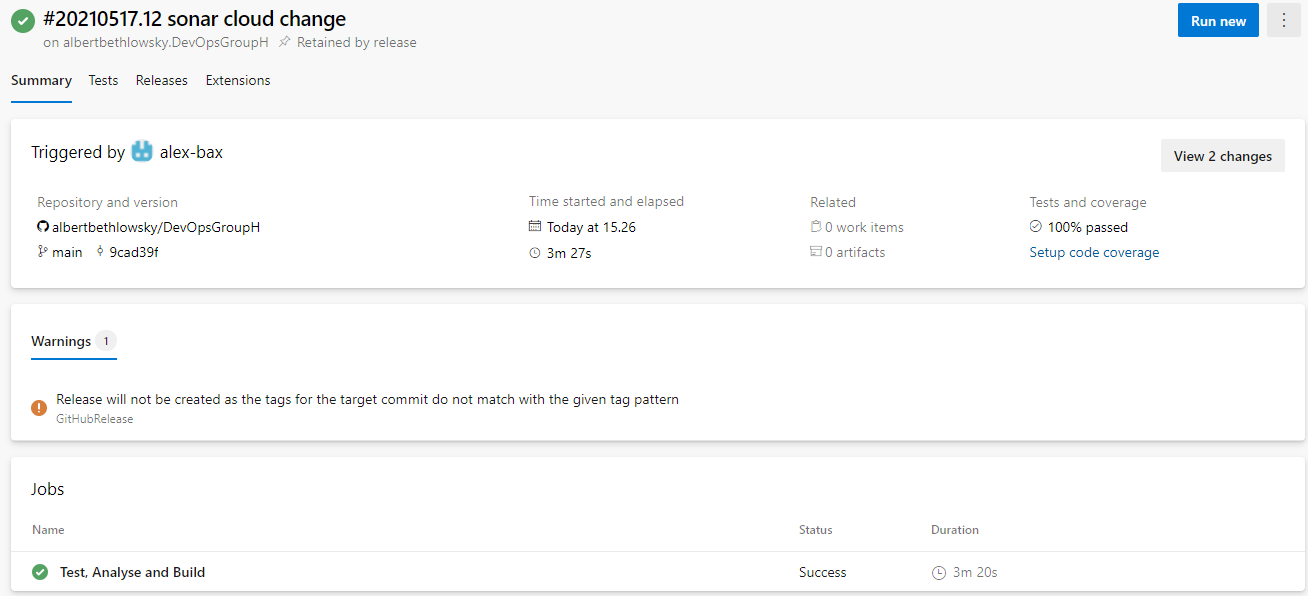
\includegraphics[width=1\textwidth]{images/pipeline-result.png}
\caption{\label{fig:res} Result of the CI chain from \texttt{azure-pipelines.yaml}}
\end{figure}
Whenever the main branch receives commits, the CI pipeline is triggered. The chain consists of one stage with the jobs executed in the order of: 
\begin{enumerate}
    \item Test and Sonar Cloud Setup and Analysis
    \item Build Image and Upload to Azure Container Registry 
    \item Make auto GitHub release (if tag added in commit)
\end{enumerate}

If testing fails the pipeline stops. No automatic git branch-merging tasks have been added. % we should have had Pipeline setup on Dev such that we don't flood main with tiny releases + be sure that dev more frequently is acceptable state + be able to check much faster if your commit is acceptable 

\subsubsection*{Continuous Delivery}
The CD pipeline, as seen in Fig. \ref{fig:release}, is responsible for pulling the latest image on ACR, and is thus triggered when a new image is pushed. ACR was chosen as the container registry for the MiniTwit image since it integrates more easily with Azure and fits for a future implementation of Kubernetes. 
\begin{figure}[H]
\centering
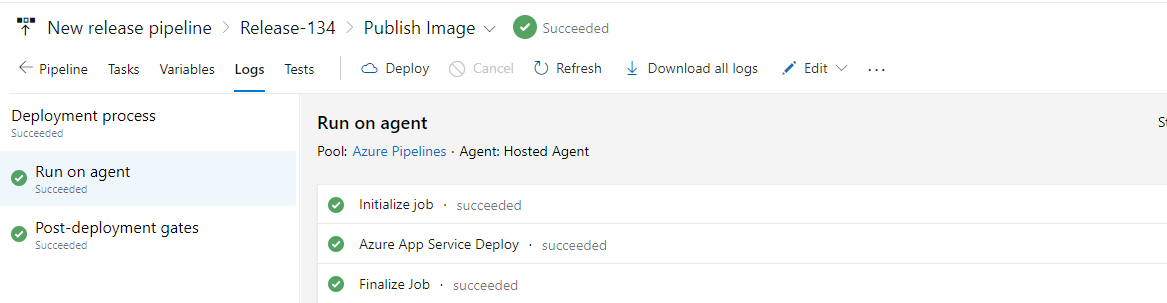
\includegraphics[width=1\textwidth]{images/devops-result.png}
\caption{\label{fig:release} CD pipeline}
\end{figure}

After having pulled, a post deployment gate is checked, in this CD chain the status of a SonarCloud Quality Gate as seen in Fig. \ref{fig:gate}. Based on the results of the SonarCloud analysis from the CI pipeline the gate is updated, and if it passes the image is deployed onto Azure. Otherwise the release will timeout after 5 minutes and fail.   

\begin{figure}[H]
\centering
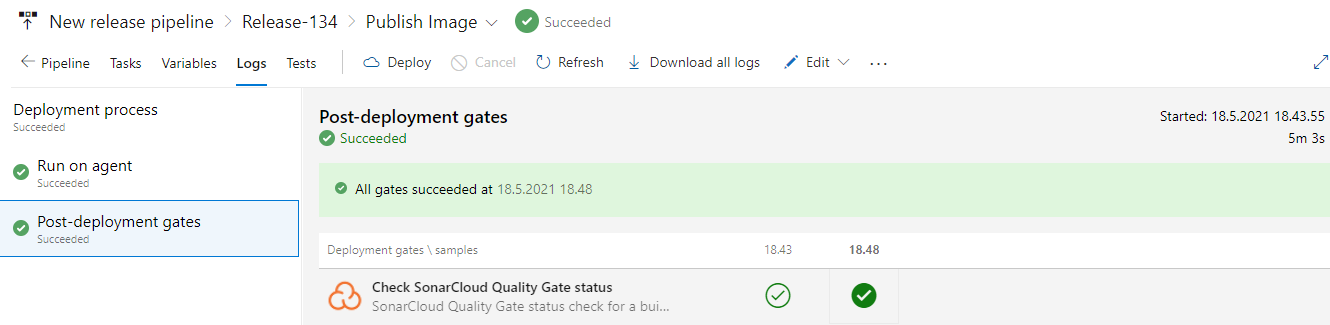
\includegraphics[width=1\textwidth]{images/post-gate.png}
\caption{\label{fig:gate} Passing SonarCloud Quality gate on the CD pipeline}
\end{figure}

% whenever a new a image is received on ACR, start Release pipeline
See \texttt{azure-pipelines.yml} for more details on the stages and tools used in the CI pipeline. Terraform will be applied to the pipeline in future iterations such that it will deploy all the services to Azure. %we ha automated the infrastructure (IaC) maintenance.  

\subsection{Applied Branching Strategy}
Throughout the project a "Long-Running Branches" strategy has been used. The \textit{main} branch has primarily been used for code releases as pull requests from \textit{development} or \texttt{.yml} pipeline changes. Smaller feature branches were merged into a \textit{development} branch, that in turn was merged into \textit{main} at the next stable release. 

The individual feature branches correspond to the issues on the task board on GitHub. Each feature branch is named after their issue number, e.g. \texttt{fea#34APIController}. Feature branches are short lived, and are deleted when done. 

Pull requests where inspected as a team or by another developer. Releases were often done manually, since that way we could a provide a description/documentation to it. This had its drawbacks, one being that it's somewhat against the DevOps idea, but also that we didn't release as often and consistently as we would have liked.   

\subsection{Applied development process and related tools}
\subsubsection*{Mono-Repository}
 We make use of a 'mono-repository', meaning that there's a unified source-code repository, that every developer can collaborate on. This seemed fitting for the size of the code base and team.

\subsubsection*{Simple Kanban board}
We used Github's Projects for task identification, specification, and planning. The board consists of the traditional Kanban setup with 'tasks', 'in progress', 'parked', and 'done' as seen the Fig. \ref{fig:kanban}. Each week we would receive a list of tasks as an assignment for the course. First, we listed them all within the 'tasks' lane. Secondly, we converted the tasks into issues and assigned group members to them. Thirdly, the tasks would be inserted into its retrospective lane. Then each Sunday we would gather up on the tasks completed on the assignment and review the code before a merge to the \textit{main} branch.

\begin{figure}[H]
\centering
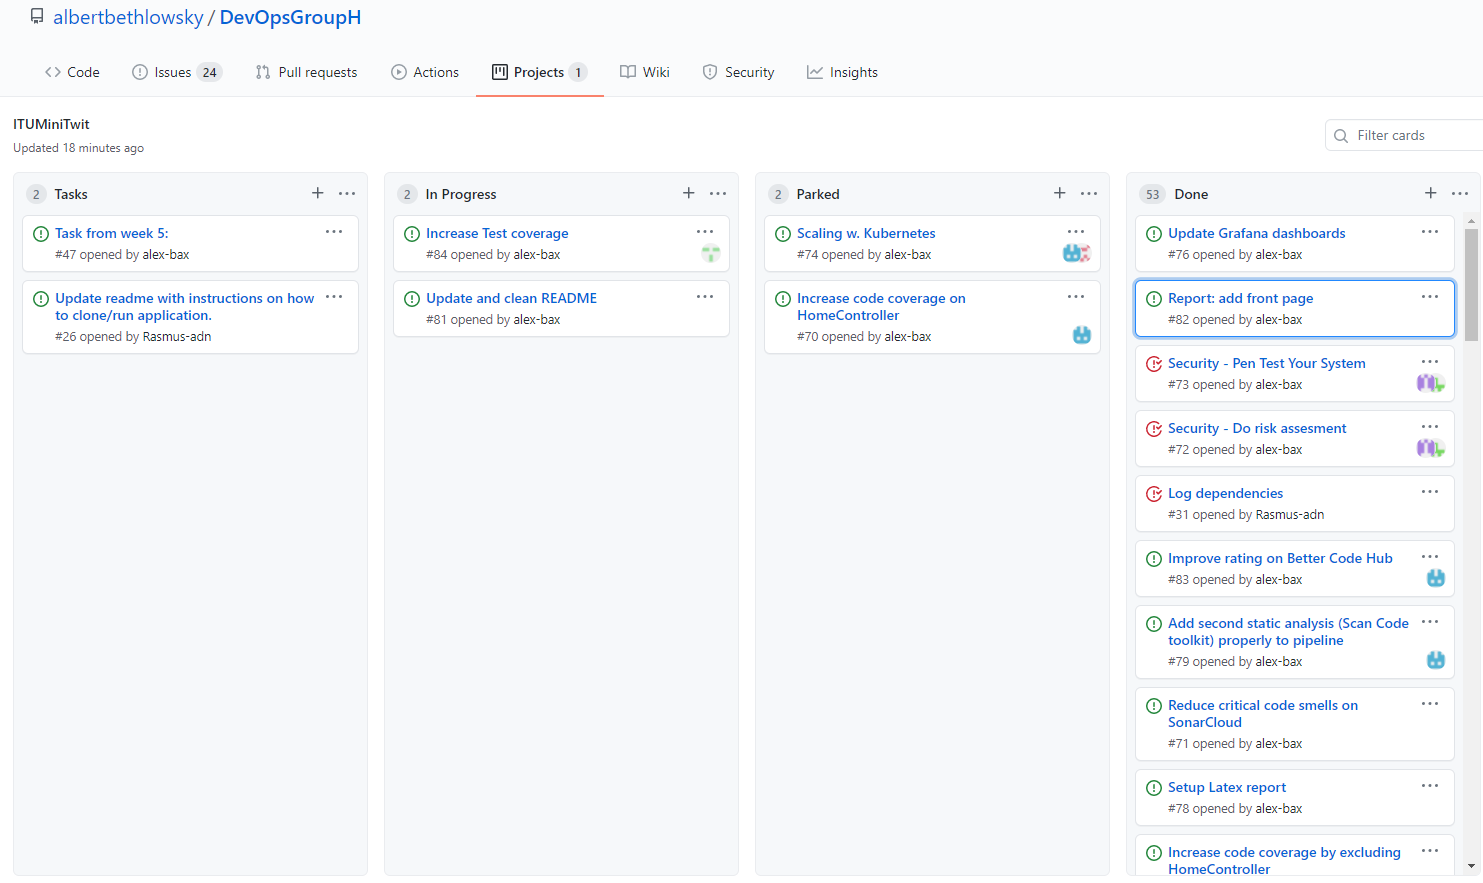
\includegraphics[width=1\textwidth]{images/kanban.png}
\caption{\label{fig:kanban} Github Project - Kanban Board}
\end{figure}
We decided to use Github Projects since we wanted to centralize our tasks in one place. Other mediums were also possible, such as monday.com, jira.com, or temgantt.com, DevOps, etc. However, we were concerned that utilizing an external solution from Github would result in poor task management.

\subsection{Monitoring}
Prometheus was chosen to scrape the data from the MiniTwit container, and Grafana to visualize it. More precisely Grafana pulls data from the Prometheus container regularly, which in turn pulls data from the application through the /metrics access point of the website. The Prometheus and Grafana images are deployed in a container on their own App Service, separate from the App Service hosting MiniTwit.

From quick research, these tools were chosen since they have good compatibility and documentation, but other alternatives to Prometheus such as DataDog could also have been chosen.

To supplement Grafana, to get insights on metrics such as RAM usage, in and out-going data bandwidth usage, thread count, etc. we used the monitoring tools available on Azure for the services hosting MiniTwit and the SQL db as seen in Fig. \ref{fig:RAM}. These stats are especially useful to determine the general load and whether or not to scale the server to meet a demand.  
\begin{figure}[H]
\centering
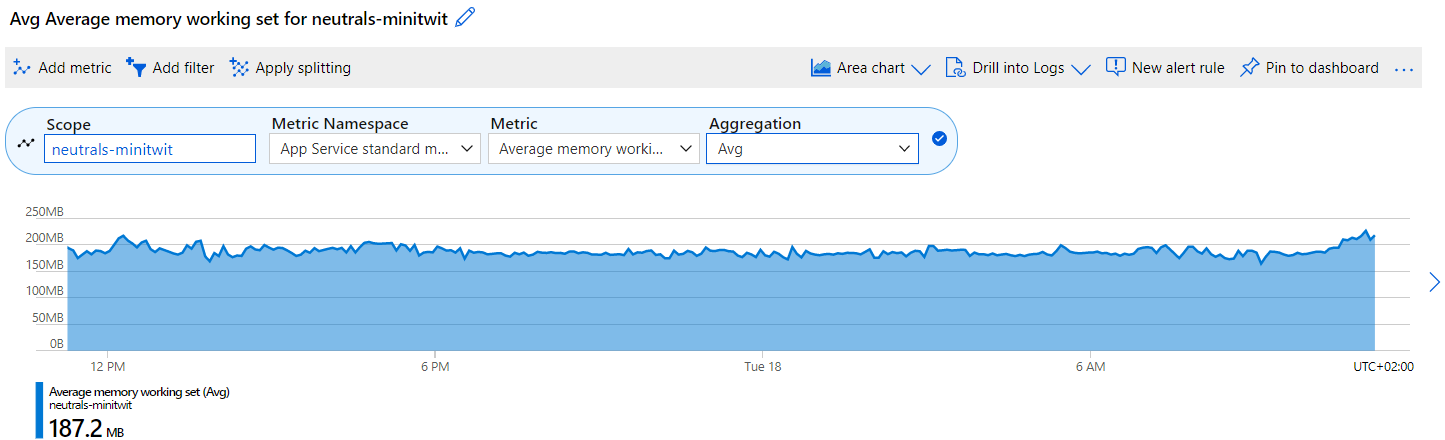
\includegraphics[width=1\textwidth]{images/azure-mem-usage.png}
\caption{\label{fig:RAM} Memory usage of MiniTwit container from the Azure App Service}
\end{figure}

\subsubsection{Dashboards on Grafana}
The \emph{Rate of http calls} dashboard shows the number of different types of HTTP responses emitted from traffic on the endpoints over time. 

For example, from inspecting Fig. \ref{fig:dashboard}, at 18.00 there was about 2.5 thousand 204 status codes sent from the server on the endpoint of the form \texttt{https://neutrals-minitwit.azurewebsites.net/msgs/Joe}
triggering method \texttt{CreateMessageByUser()} in the API.     

This includes the most common HTTP status codes 2xx, 3xx, 4xx and 5xx. It gives a general overview of how the server responds to the traffic, and has been useful to indicate error trends.

Other dashboards used are: \textit{The duration of HTTP requests}, \textit{Total no. threads} and \textit{Request currently in progress}. 

% how are they deployed? both images on the same service (from docker compose)?

\begin{figure}[H]
\centering
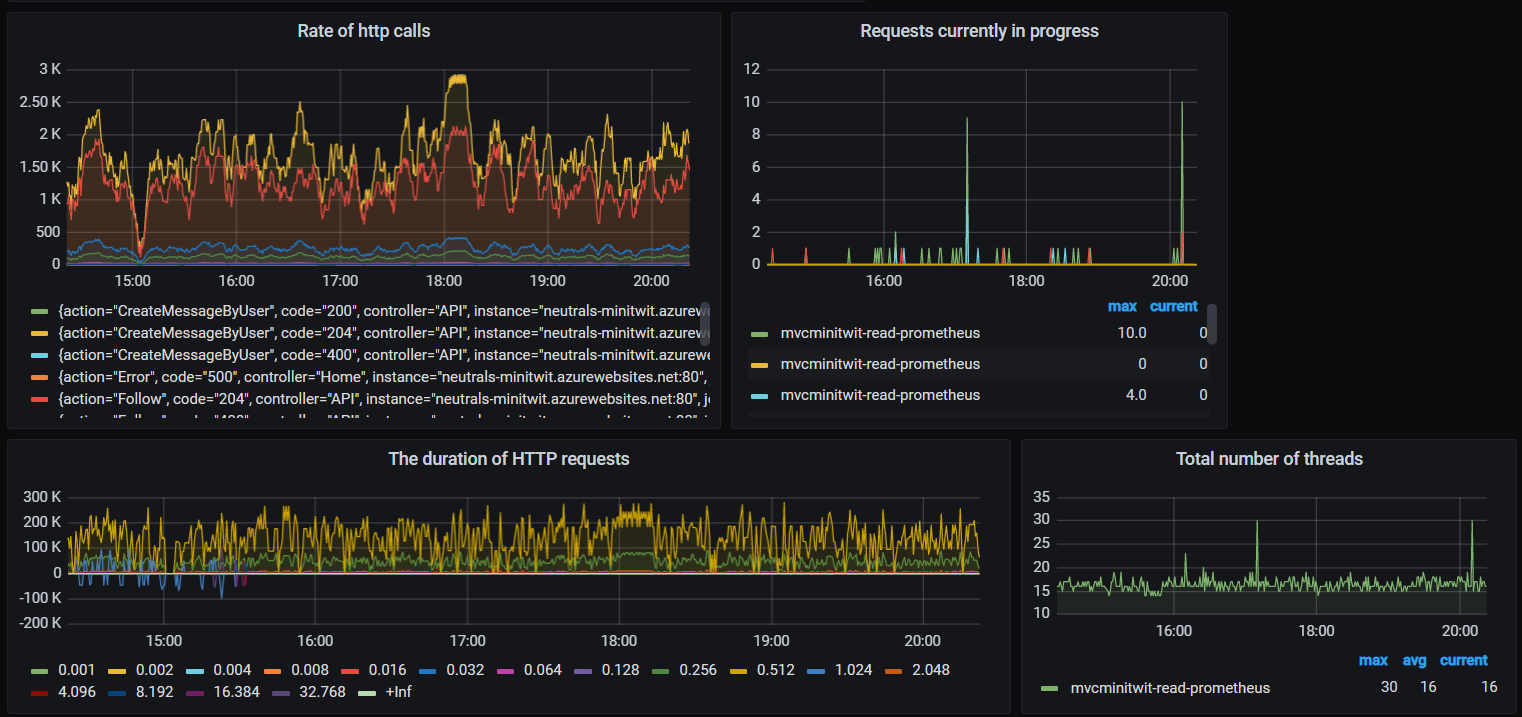
\includegraphics[width=1\textwidth]{images/dashboard.png}
\caption{\label{fig:dashboard} Grafana dashboards}
\end{figure}

In future iterations alerts from either Azure or Grafana could be considered. Also more in depth db monitoring could be implemented, since it was only shortly experimented with, tracking no. users and no. messages.

\subsection{Logging and log aggregation}
\subsubsection{Selecting a Solution}
For purposes of logging, multiple different solutions were initially discussed, one being the ELK stack introduced during the course. Even though it's very advanced, it seemed difficult to implement into our system in comparison to its benefits. 
As an alternative we investigated Promtail together with Loki. These solutions apply the same methodology as Prometheus, but in contrast captures logging information, diverting it to Loki which in turn can aggregate the log information into Grafana.

Testing this proved more difficult than expected, since working with Azure as our host gave issues with opening and forwarding ports required to utilize these programs.
In the end we decided on Serilog with Seq, further described below.

\subsubsection{Serilog}
Serilog, shown in Fig. \ref{fig:seqlog}  is injected on top of .NET's native logging infrastructure and provides simple enrichment of the log context in addition to enabling logging of custom data points captured or generated within the system.
Serilog uses a sink to continuously send log data to Datalust Seq, which is the aggregation and visualization tool used.
The "Events" tab enables search and filter on all the aggregated logs, providing a simple approach to identifying overall trends and specific errors which might have occurred in the system.

\begin{figure}[H]
\centering
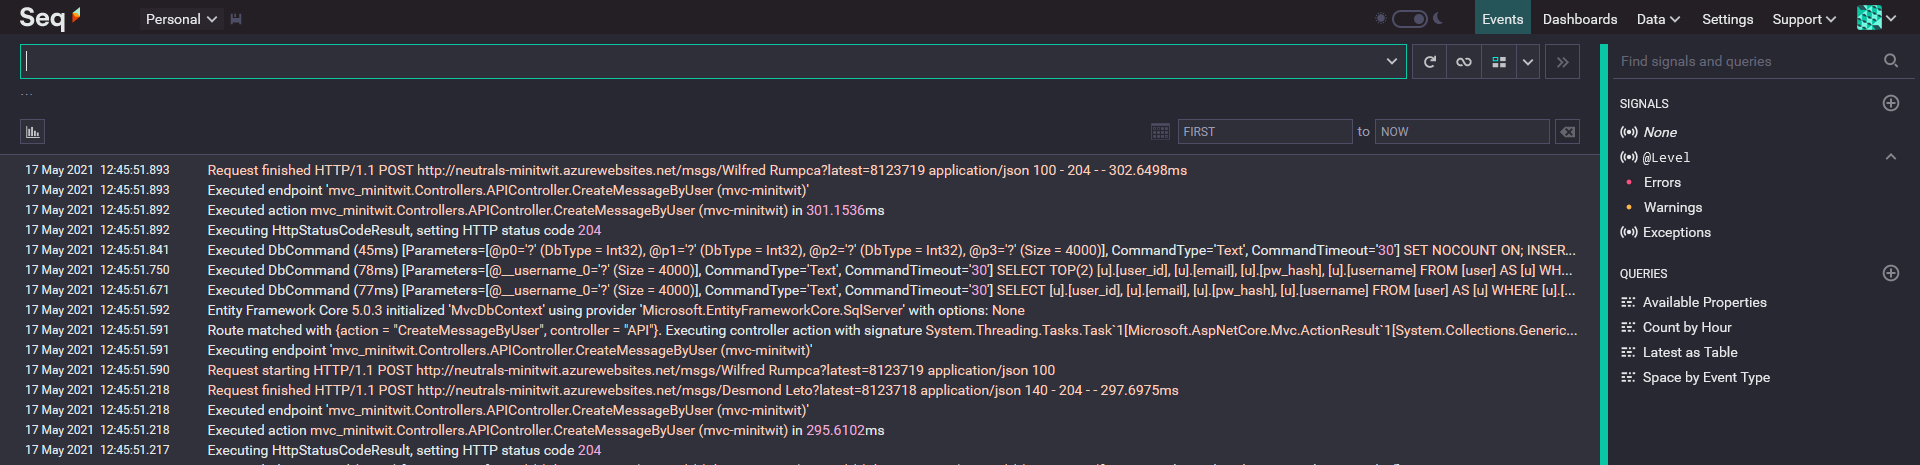
\includegraphics[width=1\textwidth]{images/DatalustSeq.PNG}
\caption{\label{fig:seqlog} Datalust Seq log}
\end{figure}

The logging we perform is primarily centered around the controllers in the system. All calls generates information in regards to actions performed, in addition user defined log entries we created to provide additional information within each call for better error-handling.

\begin{figure}[H]
\centering
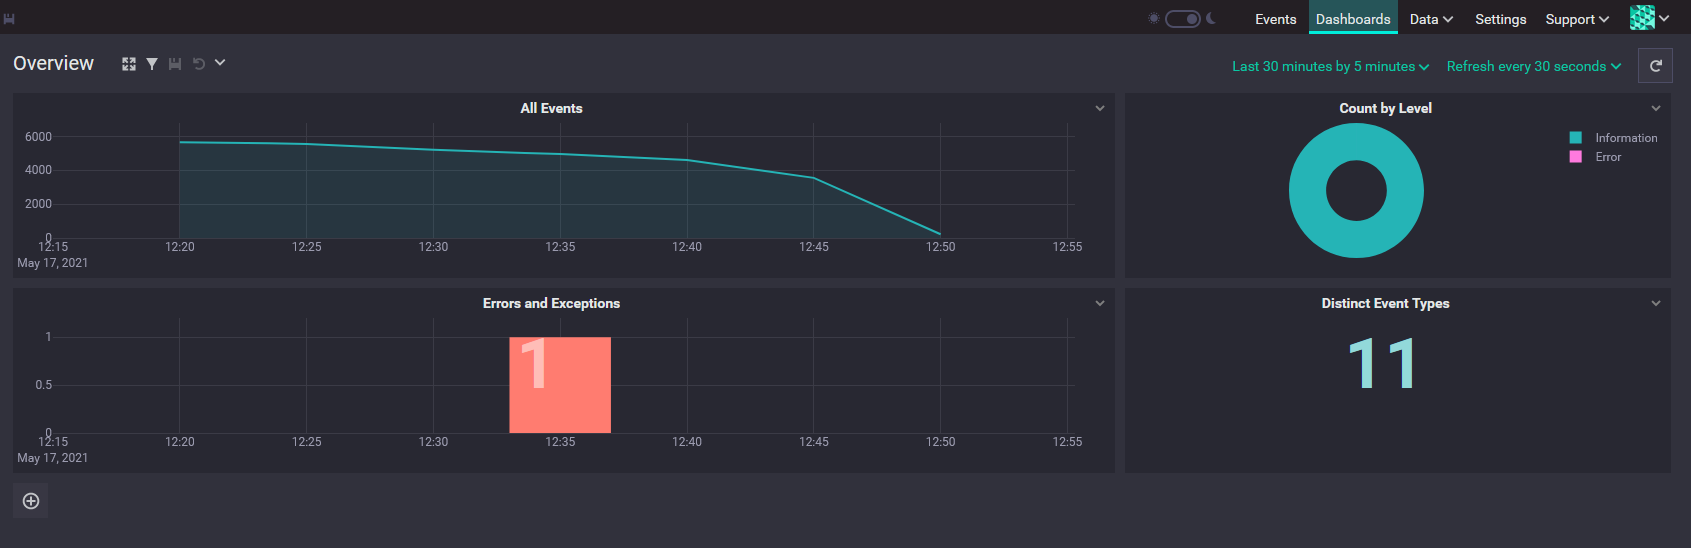
\includegraphics[width=1\textwidth]{images/DatalustSeq2.PNG}
\caption{\label{fig:seqdashboard} Datalust Seq dashboard}
\end{figure}

\subsection{Brief security assessment} 
While dotnet provides useful classes and services to write more secure code, a known security issue is that we use MD5 for hashing users passwords. MD5 is no longer considered secure as it has been cryptographically broken. Therefore using an alternative such as bcrypt or Argon2 would be safer. The most secure hashing algorithm for passwords that is currently natively supported in dotnet is PBKDF2. To solve this security concern, we could make a check when the user sign in and then rehash their password with the new algorithm.

Furthermore, we use jQuery and bootstrap, that have known security vulnerabilities. To eliminate any risks, they would have to be upgraded to the the newest version available. We consider this risk as low. 
While we use LINQ for our queries with our Entity Framework, the system is not vulnerable to SQL injection \cite{netMic}. The Entity Framework provides standards that have generally helped us eliminate different vulnerabilities. We have prevented XSS, X-frame options, and sniffing by setting security headers with the Use method directly in our Configure method in the StartUp.cs file. We have used ScanTitan \cite{titan} and Hostedscan \cite{hostedscan} to pen test our system. Our security assessment can be found in 'SecurityAssesment.md'.

\subsection{Applied scaling and load balancing strategy} 
We implemented azure's 'scale out' service which is a built-in feature that helps applications perform their best when demand changes according to Microsoft \cite{scaleout}. It enables our services to run on multiple VMs (three in our case) simultaneously and where the load will be balanced automatically. We applied this scale-out to multiple services running; Web App Services and Service Plans \cite{scaleout}. 

Moreover, we did try to establish Kubernetes services and incorporate this into our pipeline. However, we met multiple errors, both pricing tiers with azure and also authentication problems with the active directory. Simply put, ITU's active directory did not allow us to administrate Kubernetes on Azure. We also investigated the possibility of using docker swarm, but they are in a vanilla stage with azure and hence major errors occurred when trying to implement. For example, this docker swarm template for azure is being linked by Microsoft and it fails almost all of their tests \cite{dockerswarm}.


\section{Lessons learned perspective}
Throughout the lifetime of the project, numerous decisions have been made in good faith when considering the understanding of the overall project and it's technologies at those points in time. Some decisions did however result in unforeseen issues, most notable described below.
% moving db to Azure SQL - upgrade db with more DTU - 
% multiple fixes on API (adjustments in HTTP Status codes)
% should have considered indexing for the DB
\subsection{Evolution and refactoring} 
    \subsubsection{Language and Framework}
    Early on in the process, we identified that going with .NET held advantages in their offering of templates and wast majority of guidance online on multiple topics. The .NET framework spans across multiple iterations and versions  like .NETCore, .NETFramework, ASP.NET among others. Though NuGet packages are obtainable for most of the different versions, solutions to various problems were not always applicable to the system. %While not expected at any given time, but with ongoing research and due diligence, we improved at  sources were relevant and which were outdated. 

    \subsubsection{Database Management}
    Though a shift from SQLite into another DBMS was clear from the start, it became obvious, not having this transition in place in a timely manner can cause great complications as we experienced the hard way.
    During the early stages of the simulator things looked to be running as intended, we however quickly observed that this was unfortunately not the case. We identified an issue with the API unsuccessfully posting certain messages, together with following and unfollowing of users. Upon fixing the issue, we had mistakenly locked the database into the container image, thereby not being able to access any of the data stored from outside the system. 
    
    After many hours spent trying to mitigate this error, we had to admit defeat and perform our migration into another DBMS with backup data from another group. This allowed us to carry through with the necessary fixes for the API and move on with the project. Hereafter, it was clear that decoupling of the software and the database is a high priority, or as a minimum ensuring proper access to it's content before going live. 
    
    Since we are simulating a real life environment, this action resulted in the deletion of all users and messages which is far from ideal, since a backup from a third party under normal circumstances is highly unrealistic.

\subsection{Operation}
    \subsubsection{Foreshadowing}
    We define operations as the completion of the weekly assignments. Many struggles occurred at many of the weekly assignments due to a steep learning curve that had to be conquered. 
    With lacking knowledge of some of the technologies we needed to implement, most viable solutions where not always chosen, which occasionally lead to future discrepancies in our system. Initially certain functionality was implemented on standalone basis, which worked for certain aspects of the system, but in time we got better at foreshadowing; basing technology and implementation decisions not only on our current tasks, but also tasks to come.

    \subsubsection{Azure Limitations}
    Azure as a service provider comes with countless baked in solutions supporting deployment, monitoring, health checks, logging and more, providing easy setup and maintenance of simple solutions. In regards to customization of our deployment however, Azure did prove to be very difficult to work with. Azure is comprised of many tiers of pricing, granting access to various possibilities within their services. Being on a budget and on an "Azure for Students" license, made of some of the weekly requirements for the course, very difficult to complete.
    One of the most noticeable obstacles worth to mention is the inability to access certain ports.
    Azure as a default provides www.{xxx}.azurewebsites.net as access points, not enabling port specification when accessing the website. This caused a lot of issues in instances where multiple technologies needed to be embedded into a docker compose file. Ultimately in rendered us unable to run our program together with Prometheus and Grafana as an example.
    With some tinkering, we did discover the possibility of layering images on top of each other in situations where only one image needed to be displayed for usage. In the example of Prometheus and Grafana, putting Prometheus as the first image of the compose file allowed us to access the interface and confirm that traffic was flowing through correctly. Afterwards we rearranged the compose file putting Grafana as the first image, granting access to our monitoring service, while still having Prometheus functioning as intended in the background, though not accessible.
    These kinds of tweaks were required on multiple occasions, causing a lot of headaches during development and testing of different aspects in the system.
    Having to make these workarounds, despite the excitement of discovering the possibility to do so, in the end proved to cause major setbacks throughout the entire project. Trying to scale our tier to overcome these issues rapidly bleed out our funds and was therefore not deemed a suitable option.
    As a conclusion, Azure would probably not be a desirable choice on other development projects of this scale and complexity, where multiple technologies needs to be accessible, ideally through the same website / server.
    
    \subsubsection{Infrastructure as Code (IaC)}
    We tried to implement Terraform as part of our CD/CI, but we met multiple issues. We did manage to establish a working replica of our Azure resource group through Terraform together with a working Azure DevOps CD/CI pipelines, as seen in Fig. \ref{fig:terr}. However, we didn't manage to secure our various passwords and connection strings and we experienced issues with the Terraform statefile. A small typo error in the Terraform file resulted in an error which then lead to our the statefile, which is stored in a blob storage on azure, to become desynchronized, forcing us to import every single resource into a new statefile. Due to these obstacles, we decided to postpone the implementation of integrating IaC as part of our CD/CI. 
    \begin{figure}[H]
    \centering
    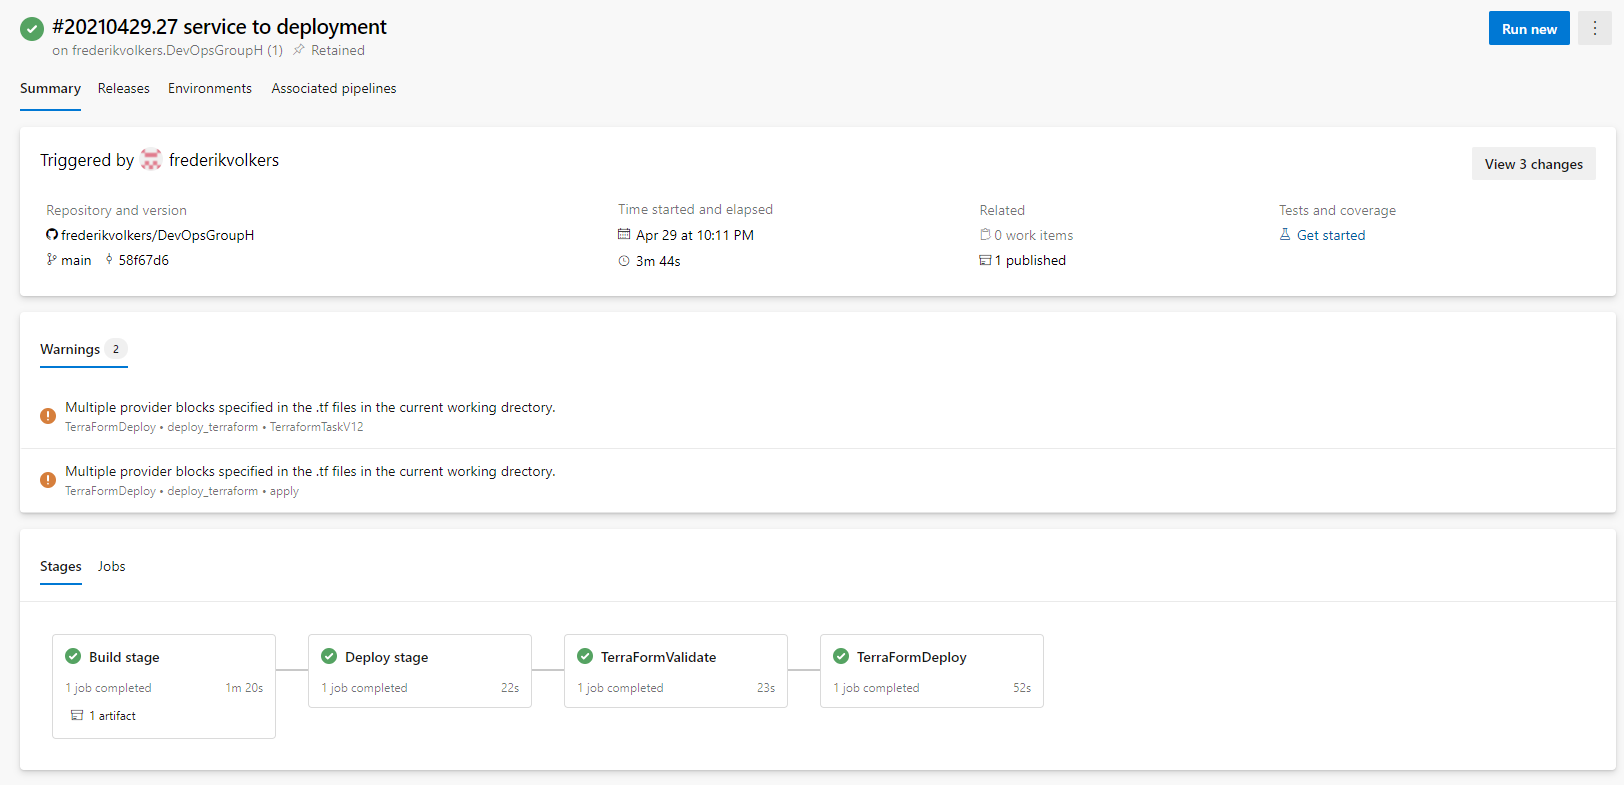
\includegraphics[width=1\textwidth]{images/terrCDCI.png}
    \caption{\label{fig:terr} Terraform Azure DevOps CD Pipeline}
    \end{figure}
        

\subsection{Maintenance}
As earlier mentioned, logging and monitoring was used to monitor the behavior of our application from where we applied maintenance accordingly. We fixed a long list of code bugs and smells with the help of the various static analysis tools e.g. SonarCloud. We also increased the coverage of our code with tests of our home and API controllers.  
As mentioned earlier, one of our biggest struggles was to send the correct status codes for the simulator. As seen in fig \ref{fig:sim}, we were the group with the largest amount of http errors. 

\begin{figure}[H]
\centering
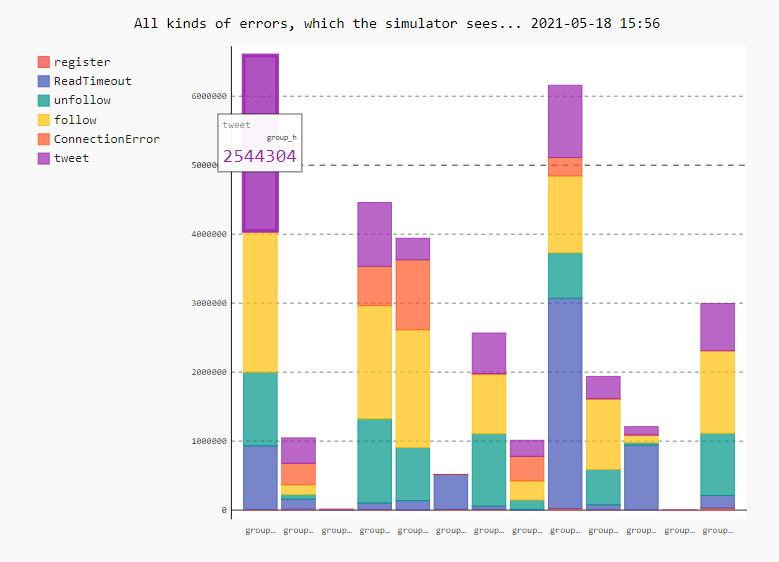
\includegraphics[width=1\textwidth]{images/simulatorerr.png}
\caption{\label{fig:sim} Simulator Errors}
\end{figure}

One reason for the large amount of http errors being created was, because of the limitations of our basic pricing tier in Azure. We solved it by vertically scaling up our database tier allowing for more Database Transaction Units (DTU's). Other reasons included: responding with the wrong response code for some time, and our API controller functioning very poorly in handling http requests. We solved the latter, by optimizing queries.


\newpage
\bibliographystyle{acm}
\bibliography{sample}

\end{document}